%%%%%%%%%%%%%%%%%%%%%%%%%%%%%%%%%%%%%%%%%
% Beamer Presentation
% LaTeX Template
% Version 1.0 (10/11/12)
%
% This template has been downloaded from:
% http://www.LaTeXTemplates.com
%
% License:
% CC BY-NC-SA 3.0 (http://creativecommons.org/licenses/by-nc-sa/3.0/)
%
%%%%%%%%%%%%%%%%%%%%%%%%%%%%%%%%%%%%%%%%%

%----------------------------------------------------------------------------------------
%	PACKAGES AND THEMES
%----------------------------------------------------------------------------------------

\documentclass[xcolor=table]{beamer}

\usepackage{tikz}
\setbeamertemplate{background canvas}{\begin{tikzpicture}\node[opacity=.3]{
\includegraphics
		[width=\paperwidth]{imagenes/background2.png}};\end{tikzpicture}}

%\setbeamertemplate{background}
%{
\includegraphics[width=\paperwidth,height=\paperheight,keepaspectratio]{imagenes/background2.png}}

\mode<presentation> {

% The Beamer class comes with a number of default slide themes
% which change the colors and layouts of slides. Below this is a list
% of all the themes, uncomment each in turn to see what they look like.

%\usetheme{default}
%\usetheme{AnnArbor}
%\usetheme{Antibes}
%\usetheme{Bergen}
%\usetheme{Berkeley}
%\usetheme{Berlin}
%\usetheme{Boadilla}
%\usetheme{CambridgeUS}
%\usetheme{Copenhagen}
%\usetheme{Darmstadt}
%\usetheme{Dresden}
%\usetheme{Frankfurt}
%\usetheme{Goettingen}
%\usetheme{Hannover}
%\usetheme{Ilmenau}
%\usetheme{JuanLesPins}
%\usetheme{Luebeck}
\usetheme{Madrid}
%\usetheme{Malmoe}
%\usetheme{Marburg}
%\usetheme{Montpellier}
%\usetheme{PaloAlto}
%\usetheme{Pittsburgh}
%\usetheme{Rochester}
%\usetheme{Singapore}
%\usetheme{Szeged}
%\usetheme{Warsaw}

% As well as themes, the Beamer class has a number of color themes
% for any slide theme. Uncomment each of these in turn to see how it
% changes the colors of your current slide theme.

%\usecolortheme{albatross}
%\usecolortheme{beaver}
%\usecolortheme{beetle}
%\usecolortheme{crane}
%\usecolortheme{dolphin}
%\usecolortheme{dove}
%\usecolortheme{fly}
%\usecolortheme{lily}
%\usecolortheme{orchid}
%\usecolortheme{rose}
%\usecolortheme{seagull}
%\usecolortheme{seahorse}
%\usecolortheme{whale}
%\usecolortheme{wolverine}

%\setbeamertemplate{footline} % To remove the footer line in all slides uncomment this line
%\setbeamertemplate{footline}[page number] % To replace the footer line in all slides with a simple slide count uncomment this line

%\setbeamertemplate{navigation symbols}{} % To remove the navigation symbols from the bottom of all slides uncomment this line
}

\usepackage{graphicx} % Allows including images
\usepackage[spanish]{babel}
\usepackage{booktabs} % Allows the use of \toprule, \midrule and \bottomrule in tables
 \usepackage{multirow}


%----------------------------------------------------------------------------------------
%	TITLE PAGE
%----------------------------------------------------------------------------------------

\title[Perdida de Carbono]{Metodolog\'ia autom\'atica para estimar p\'erdida de	carbono a trav\'es de procesamiento de im\'agenes
	satelitales. Caso de uso Chaco Paraguayo} % The short title appears at the bottom of every slide, the full title is only on the title page

\author{Santiago Vera Aquino} % Your name
\institute[FP-UNA] % Your institution as it will appear on the bottom of every slide, may be shorthand to save space
{
Universidad Nacional de Asunci\'on \\ % Your institution for the title page
Facultad Polit\'ecnica \\
Ingenier\'ia en Inform\'atica \\
\medskip
\textit{Proyecto Final de grado} % Your email address
}
\date{\today} % Date, can be changed to a custom date

\begin{document}

\begin{frame}
\titlepage % Print the title page as the first slide
\end{frame}

%------------------------------------------------

	\begin{frame}
		\frametitle{Contenido}
		\tableofcontents[currentsection,currentsubsection]
	\end{frame}

%------------------------------------------------	

\begin{frame}
\frametitle{Planteamiento del problema}

De entre los servicios ambientales que proporcionan los bosques, la captura de carbono ser\'a determinante para disminuir el calentamiento global y estabilizar el cambio clim\'atico producidos por el incremento en la atm\'osfera de los llamados Gases de Efecto Invernadero (GEI).\\~\\
Paraguay es un pa\'is que basa su econom\'ia en la agricultura y la ganader\'ia extensiva, actividades que han afectado al recurso forestal dando como resultado extensas \'areas deforestadas y degradadas.\\~\\

\end{frame}

%------------------------------------------------
\begin{frame}
	\frametitle{Motivac\'ion}
REDD+ es una iniciativa que tiene como objetivo reducir la p\'erdida de bosques, las actividades REDD+ evitan p\'erdidas como emisiones de gases de efecto invernadero (conservaci\'on, no deforestaci\'on, no degradaci\'on), mantienen el dep\'osito o stock de carbono (conservaci\'on, gesti\'on sostenible), o incrementan el dep\'osito por su efecto de retenci\'on o sumidero de carbono (conservaci\'on, restauraci\'on, gesti\'on sostenible).\\~\\
	
El Paraguay se ha embarcado en el proceso de preparaci\'on para Reducir la Deforestaci\'on y Degradaci\'on forestal (REDD+)   a fin de disminuir las emisiones de CO2, conservar los bosques y su biodiversidad, por tanto se busca elaborar una estrategia nacional, con pol\'iticas socios ambientales y econ\'omicos viables, as\'i como el desarrollo de capacidades.
	
	
\end{frame}

%------------------------------------------------
\begin{frame}
	\frametitle{Motivac\'ion}
As\'i para medir los beneficios de carbono de un proyecto REDD+, es necesario calcular la cantidad de carbono almacenado en el bosque en cuesti\'on y luego predecir la cantidad de carbono que se podr\'ia conservar si se detiene o reduce la deforestaci\'on y la degradaci\'on forestal.\\~\\
	
La mayor\'ia de las investigaciones para estimar y mapear la biomasa en bosques se centran en las t\'ecnicas de Sensores Remotos; debido a las grandes extensiones de las \'areas de estudio, la dificultad de acceder a las mismas, el alto costo del establecimiento de las parcelas de inventario y su limitada utilidad debido a la variabilidad natural espacial de la biomasa forestal. Por ello la necesidad de crear metodolog\'ias que ayuden al monitoreo de forma din\'amica y barata nos lleva al desarrollo de herramientas libres que permitan estimar focos de alerta para la toma de acciones y controles m\'as rigurosos a tiempo.
	
	
\end{frame}

%------------------------------------------------


\begin{frame}
	\frametitle{Antecedentes}
	Sassan Saatchi del Jet Propulsion Laboratory, California Institute of Technology, en colaboraci\'on con la NASA, realiza investigaciones que se centra en diversos aspectos del ciclo de carbono terrestre. Usa una combinaci\'on de sensores remotos y datos in situ para mapear el carbono almacenado en los bosques, para cuantificar sus cambios con respecto a las perturbaciones humanas y naturales, tambi\'en estimar el dinamismo de las interacciones e impactos clim\'aticos. 
	
	
\end{frame}

%------------------------------------------------


\begin{frame}
	\frametitle{Antecedentes}

	Existen trabajos realizados por estudiantes de la Facultad de Ciencias Agrarias - UNA como proyecto de grado en zonas especificas como la reserva de la biosfera del Chaco, Parque Nacional San Rafael y el Parque Nacional Defensores del chaco, todos ellos en la regi\'on Occidental del Paraguay. Implementan una metodolog\'ia base hecha en el marco denominado \textit{Desarrollo del estudio de linea de base para el sitio piloto Bosque atl\'antico de Alto Paran\'a. (BAAPA)} realizado por el Paraguay Land Use (ParLu), el cual es una iniciativa de World Wildlife Fund (WWF)	Paraguay y WWF Alemania que apoya las iniciativas REDD+ en Paraguay, generando mapas de stock de carbono y los correspondientes mapas de cobertura y de Deforestaci\'on 2000\textendash2005 y 2005\textendash2011 a partir de muestreos de parcelas in situ y clasificaciones supervisadas con la ayuda de aplicaciones con licencias de car\'acter propietario, todo esto conjuntamente con la  Carrera de Ingenier\'ia Forestal de la Facultad de Ciencias Agrarias perteneciente a la Universidad Nacional de Asunci\'on.
	
	
\end{frame}

%------------------------------------------------


\begin{frame}
	\frametitle{Antecedentes}
	
Un estudio realizado por por University of Maryland Institute for Advanced Computer Studies denominado Forest Cover Change in Paraguay, nos muestra el cambio de vegetaci\'on estimado en todo el pais utilizando un m\'etodo iterativo de etiquetado de cambio por clusterizaci\'on supervisada. El trabajo detecta cambios de los a\~{n}os 1992 al 2000, donde aparte de proveer un etiquetado de cambios de vegetaci\'on fue realizada con im\'agenes de mejor resoluci\'on espacial, de acceso libre, generando informaci\'on m\'as precisa.
	
\end{frame}

%------------------------------------------------
\begin{frame}
	\frametitle{Formulaci\'on general del Proyecto}
	\begin{block}{Problema u Oporunidad}
		\begin{itemize}
			\item La informaci\'on referente al secuestro de carbono es muy escasa y discontinua en todo el pa\'is, m\'as aun en zonas del chaco, lo cual dificultad la detecci\'on y soluci\'on de las problem\'aticas que acarrea la p\'erdida de carbono.
			\item La generaci\'on de informaci\'on ambiental es muy costosa en el Paraguay, debido a no contar con una metodología pr\'actica  que agilice los procesos utilizando informaciones p\'ublicas y herramientas libres.
		\end{itemize}
	\end{block}
		\begin{block}{Soluci\'on propuesta por el proyecto de investigaci\'on}
			\begin{itemize}
				\item La soluci\'on propuesta por el proyecto es dise\~{n}ar e implementar una metodolog\'ia que ayude a estimar y comparar  el contenido de carbono en una regi\'on de manera pr\'actica y con un flujo continuo en series de tiempo.
			\end{itemize}
		\end{block}
	
\end{frame}

%------------------------------------------------
%------------------------------------------------

\begin{frame}
	\frametitle{Formulaci\'on general del Proyecto}
	\begin{block}{Hip\'otesis del proyecto}
		\begin{itemize}
			\item La idea consiste en aplicar operaciones de procesamiento de im\'agenes para realizar una comparaci\'on multitemporal de im\'agenes espectrales e \'indices derivados de ellas, previo a la clasificaci\'on de vegetaci\'on para la estimaci\'on de p\'erdida de carbono.
		\end{itemize}
	\end{block}
	
\end{frame}
%------------------------------------------------

\begin{frame}
	\frametitle{Objetivos del proyecto}
	\begin{block}{Objetivos Generales}
		\begin{itemize}
			\item Desarrollar una metodolog\'ia de an\'alisis de im\'agenes espectrales multitemporales para la generaci\'on de indicadores  respecto a cambios de contenido de carbono en zonas del Chaco Paraguayo.
		\end{itemize}
	\end{block}
	\begin{block}{Objetivos Espec\'ifico}
		\begin{itemize}
			\item Estudiar el estado del arte en teledetecci\'on aplicada en el medio ambiente.
			\item Realizar detecciones de cambio automatizada dentro del \'area de estudio a trav\'es de la Teledetecci\'on y un SIG.
			\item Realizar	proyecciones de acuerdo a las tendencias observadas en los resultados.
			\item Aportar 	informaci\'on ambiental en la zona del chaco, para futuros estudios e investigaciones.
		\end{itemize}
	\end{block}
	
\end{frame}

%------------------------------------------------
%------------------------------------------------
\begin{frame}\frametitle{Carbono y Biomasa}

La biomasa es aquella materia org\'anica de origen vegetal o animal, incluyendo los residuos y desechos org\'anicos, susceptible de ser aprovechada energ\'eticamente. Las plantas transforman la energ\'ia radiante del sol en energ\'ia qu\'imica a trav\'es de la fotos\'intesis, y parte de esta energ\'ia queda almacenada en forma de materia org\'anica.\\~\\
El conocer la cantidad de biomasa por \'arbol en cada una de las especies que crecen en el bosque, permite estimar la cantidad de carbono que contiene un grupo de \'arboles, un rodal o el bosque en su totalidad, ya que al multiplicar la cantidad de biomasa por un factor de conversi\'on, obtenido por muestreo, se logra determinar la cantidad de carbono.

\end{frame}
%------------------------------------------------
\begin{frame}\frametitle{Teledetecci\'on}

		La teledetecci\'on es la ciencia y arte de obtener informaci\'on acerca de la superficie de la Tierra sin entrar en contacto con ella. Esto se realiza detectando y grabando la energ\'ia emitida o reflejada y procesando, analizando y aplicando esa informaci\'on.\\~\\
		Para producirse la teledetecci\'on, se requiere de la interacci\'on de tres componentes principales: flujo energ\'etico, objeto observado y un sensor.

\end{frame}


%------------------------------------------------
%------------------------------------------------
\begin{frame}\frametitle{Teledetecci\'on}
\textbf{El espectro electromagn\'etico}\\~\\
Aunque los valores de longitudes de onda son continuos, se establece una serie de bandas en donde la radiación electromagnética manifiesta un comportamiento similar. El espectro electromagnético es la organización de estas bandas de longitudes de onda o frecuencia.
Las bandas m\'as empleadas en teledetecci\'on son las siguientes:
\begin{itemize}
\item Espectro visible (400 nm a 700 nm)
\item Infrarrojo próximo: (700 nm a 1300 nm)
\item Infrarrojo medio: (1,3 um a 8 um)
\item Infrarrojo lejano o térmico: (8 um a 14 um)
\item Microondas: (a partir de 1 um)
\end{itemize}

	
\end{frame}
%------------------------------------------------
%------------------------------------------------
\begin{frame}\frametitle{Teledetecci\'on}
	\textbf{Firmas espectrales}\\~\\	

\begin{figure}
\centering
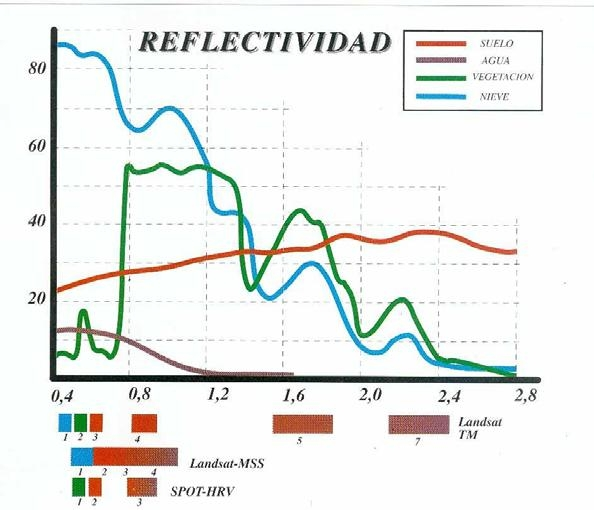
\includegraphics[width=0.7\linewidth]{imagenes/espectral}
\caption{Firma espectral de diferentes coberturas}
\label{fig:espectral}
\end{figure}

\end{frame}

%------------------------------------------------
\begin{frame}\frametitle{Teledetecci\'on y Biomasa }
	
	La biomasa es un par\'ametro que no se puede obtener directamente desde im\'agenes de sat\'elite, de hecho no se puede medir directamente ni siquiera en campo. Con la teledetecci\'on se obtienen im\'agenes que permiten analizar la reflectividad de los lugares en diferentes regiones del espectro electrom\'agnético y esa informaci\'on se puede transformar en ecuaciones que estimen par\'ametros biol\'ogicos de esas regiones (y a su vez, esos par\'ametros biol\'ogicos transformarlos en biomasa).
	
	
\end{frame}
%------------------------------------------------



%------------------------------------------------
\begin{frame}\frametitle{Sensores Remotos}
Son sistemas de adquisici\'on de informaci\'on de la superficie terrestre, soportados sobre diferentes tipos de plataformas (terrestres, a\'ereas o satelitales), funcionan a trav\'es de la captura de la energ\'ia reflejada o radiada por la superficie, ya
sea emitida por el sol (sensores pasivos) o por el mismo sensor (sensores activos). \\~\\
Los productos que se obtienen al emplear estas herramientas son diversos y de diferentes especificaciones, entre ellos los m\'as conocidos son las fotografías aéreas y las im\'agenes de sat\'elite
	
\end{frame}
%------------------------------------------------

\begin{frame}\frametitle{Resoluciones de un sensor}

	\begin{itemize}
		\item Resoluci\'on espacial
		\item Resoluci\'on espectral
		\item Resoluci\'on radiom\'etrica
		\item Resoluci\'on temporal
	\end{itemize}
	
	
\end{frame}

%------------------------------------------------
\begin{frame}\frametitle{Im\'agenes satelitales}
	La imagen satelital consiste de un arreglo matricial bidimensional de elementos de imagen llamados p\'ixeles, ordenados en filas y columnas formando una malla las im\'agenes organizadas de esta manera son conocidas como im\'agenes r\'aster. Cada p\'ixel representa un \'area de superficie sobre la tierra. Un p\'ixel tiene un valor de intensidad y una ubicaci\'on en la imagen bidimensional.
	
\end{frame}
%------------------------------------------------

%------------------------------------------------
\begin{frame}\frametitle{Sat\'elite Landsat}
	Este sat\'elite, dotado de sensores empleados en teledetecci\'on fue dise\~{n}ado con
	el fin de tener datos sobre el recurso terrestre, en base a este objetivo se dise\~{n}aron las
	resoluciones para adaptarse a este fin. El sensor Landsat TM thematic mapper9
	dise\~{n}ado directamente como su nombre lo indica para la cartograf\'ia tem\'atica, es un
	equipo de barrido multi\textendash sespectral. La tarea principal de este sensor es el de control
	medioambiental, la evaluaci\'on de desastres, la explotaci\'on del suelo y la
	planificaci\'on regional, la cartograf\'ia, la administraci\'on de pastizales y la exploraci\'on
	petrolera y de minerales.
	
\end{frame}
%------------------------------------------------

%------------------------------------------------
\begin{frame}\frametitle{\'Indice de vegetaci\'on diferencial normalizada (NVDI)}
	Los \'indices espectrales muestran un aspecto o caracter\'istica del terreno a partir de la informaci\'on radiom\'etrica contenida en las im\'agenes multiespectrales.\\~\\
	El \'indice diferencial de vegetaci\'on normalizado (NDVI) ha sido ampliamente reconocido como uno de los m\'as \'utiles para el estudio de caracter\'isticas de la biosfera terrestre y su din\'amica, a nivel global, regional y local. El NDVI es un \'indice espectral normalizado que toma valores en el intervalo $[1,-1]$ y se extrae de las bandas correspondientes al rojo $B_{R}$ e infrarrojo pr\'oximo $B_{IRc}$ seg\'un la siguiente expresi\'on:
	\begin{equation}
	NDVI=\dfrac{B_{IRc}-B_{R}}{B_{IRc}+B_{R}}
	\end{equation}

\end{frame}
%------------------------------------------------

%------------------------------------------------
\begin{frame}\frametitle{Preprocesamiento de im\'agenes satelitales}
Consiste en el procesamiento inicial de los datos crudos para corregir las distorsiones radiom\'etricas y geom\'etricas de la imagen y eliminar el ruido.  Las distorsiones radiom\'etricas obedecen a mecanismos que alteran los valores de brillo de  los pixeles y se deben fundamentalmente a interferencias atmosf\'ericas y a efectos asociados  a instrumentaci\'on. Las correcciones atmosf\'ericas constituyen un problema muy complejo si se quieren aplicar  sobre la base de modelos f\'isicos del comportamiento de las radiaciones. En efecto, estos modelos tienen el m\'erito de su rigor cient\'ifico, precisi\'on y aplicabilidad a un amplio rango de circunstancias, pero suelen exigir complejos programas de computadora así como información meteorol\'ogica detallada relativa a las condiciones en que se registr\'o la escena. Esta informaci\'on es muy difícil de obtener y podemos decir que la aplicaci\'on rutinaria de estos modelos actualmente no es posible.  Una aproximaci\'on sencilla y pr\'actica a la correcci\'on del efecto atmosf\'erico se basa en la  consideraci\'on de los histogramas de las im\'agenes espectrales.
\end{frame}
%------------------------------------------------
%------------------------------------------------
\begin{frame}\frametitle{Proceso de detecci\'on de cambios}
Los m\'etodos de comparaci\'on multitemporal, generan una imagen
(\'indice de cambios) que representa el grado de cambio entre dos situaciones temporales;
las celdas de la imagen resultante, contienen una variable continua de tipo cuantitativo. Se
requiere de t\'ecnicas de segmentaci\'on y clasificaci\'on para cuantificar el
grado de cambio asociado a cada celda; convertir una variable cuantitativa, en una variable
cualitativa.
\end{frame}
%------------------------------------------------



\begin{frame}\frametitle{Metodolog\'ia }
\textbf{M\'etodos de comparaci\'on basados en operaciones o algoritmos de \'algebra de imagen}\\~\\	
Estos m\'etodos, se basan en operaciones sencillas por lo que se pueden implementar en un proceso no supervisado y se estructuran en tres etapas generales: pre-proceso, proceso de asignación (criterios de decisión) y post-proceso.	
	
\end{frame}
%------------------------------------------------
\begin{frame}\frametitle{Metodolog\'ia }
	\textbf{Datos disponibles}\\~\\	
	Se dispone de im\'agenes Landsat 5 y 7 con Path/Row 228/76 de fechas 1/26/1992 y 8/17/1999 para las validaciones de precisic\'ion y control de calidad, junto con una imagen de un estudio elaborado por University of Maryland Institute for Advanced Computer Studies respecto al cambio de vegetac\'ion.
	Para el calculo del Umbral de vegetaci\'on se utilizaron una imagen landsat 5 del a\~{n}o 1986 junto con MODIS Vegetation Continuous Fields elaborado por University of Maryland, Department of Geography and NASA, del a\~{n}o 2000.
	Por \'ultimo para la determinaci\'on del carbono una imagen landsat 7 y el mapa de carbono elaborado por California Institute of Technology perteneciente a la NASA, las dos im\'agenes del 2001.
	
\end{frame}
%------------------------------------------------

\begin{frame}\frametitle{Metodolog\'ia - Pre-Proceso}
	\textbf{Correci\'on Geom\'etricas}\\~\\	
Los ajustes geom\'etricos engloban toda serie de operaciones aplicadas sobre las	im\'agenes iniciales que permitan el co-registro espacial de estas; de manera que las celdas situadas en la misma posici\'on en cada imagen, se asocia a la misma área del terreno.
	
	
\end{frame}
%------------------------------------------------

\begin{frame}
	\frametitle{Metodolog\'ia - Pre-Proceso}
	\textbf{Correcci\'on radiom\'etrica}\\~\\	
	Se busca optimizar el proceso para mejorar la semejanza entre im\'agenes aplicando m\'etodos de normalizaci\'on a partir de los par\'ametros estad\'isticos de la imagen.\\~\\
	Una variable tipificada \textit{(Z)} se define para una distribuci\'on est\'andar del tipo \textit{N(0,1)} seg\'un la expresión:
	\begin{equation}
	Z=\dfrac{VD-\mu}{\sigma}
	\end{equation}
	Aplicando este concepto sobre cada una de las dos im\'agenes, se pueden comparar siendo ambas distribuciones estandarizadas:
	
\end{frame}
%------------------------------------------------
\begin{frame}
	\frametitle{Metodolog\'ia - Pre-Proceso}
	\begin{equation}
	\dfrac{VD_{1}-\mu_{1}}{\sigma_{1}}=\dfrac{VD_{2}-\mu_{2}}{\sigma_{2}}
	\end{equation}
	Para su aplicación pr\'actica, se puede transformar el valor digital (VD) de las celdas de la imagen 1, para que se asemeje al VD de las de la imagen 2, expresi\'on:
	\begin{equation}
	VD_{Norm}=\mu_{2}+\dfrac{\sigma_{2}}{\sigma_{1}}\cdot(VD_{1}-\mu_{1})
	\end{equation}
	Así se puede definir una relaci\'on lineal entre las dos distribuciones; aplicando una normalizaci\'on radiom\'etrica estad\'istica, los par\'ametros de la transformaci\'on \textit{m12} y \textit{n12} se definen seg\'un se indica en la expresi\'on:

	
\end{frame}
%------------------------------------------------
%------------------------------------------------
\begin{frame}
	\frametitle{Metodolog\'ia - Pre-Proceso}
	\begin{equation}
	n_{12}=\mu_{2}-\dfrac{\sigma_{2}}{\sigma_{1}}\cdot\mu_{1} ; 
	m_{12}=\dfrac{\sigma_{2}}{\sigma_{1}} \Rightarrow VD_{Norm}=m_{12}\cdot VD_{1}+n_{12}
	\end{equation}
	\begin{figure}
\centering
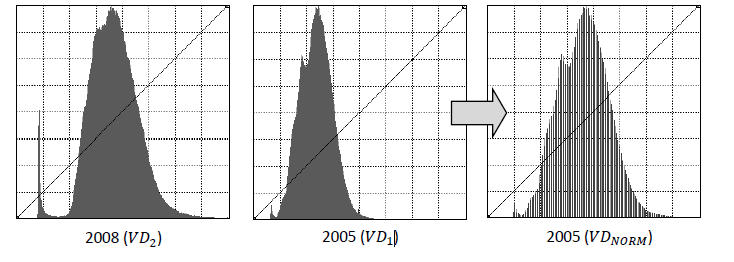
\includegraphics[width=0.8\linewidth]{imagenes/normalizacion}
\caption{Normalizaci\'on Radiom\'etrica}
\label{fig:normalizacion}
\end{figure}
	
\end{frame}



%------------------------------------------------
\begin{frame}
	\frametitle{Metodolog\'ia - Proceso de Detecci\'on de cambio}
	\textbf{Comparaci\'on multitemporal}\\~\\	
	La diferencia de imagen por ser el m\'etodo más simple, f\'acil de interpretar y directo; se suele aplicar combinada con la extracci\'on de \'indices espectrales.
	\begin{equation}
	I_{Dif.}=VD_{final}-VD_{inicial}
	\end{equation}

\end{frame}
%------------------------------------------------
\begin{frame}
	\frametitle{Metodolog\'ia - Proceso de Detecci\'on de cambio}
	\textbf{Criterios de decisi\'on. Umbralizaci\'on.}\\~\\	
Se propone, como criterios de decisi\'on, aplicar m\'etodo de discriminaci\'on basado en los par\'ametros estad\'isticos del \'indice de cambio entre la secuencia temporal de im\'agenes:
	\begin{equation}
U=\mu\pm n\cdot\sigma
	\end{equation}
	Donde, el valor de umbral entre cambio/no cambio $(U)$ se estima en funci\'on de los par\'ametros estad\'isticos $(\mu,\sigma) $ y un coeficiente de tolerancia $ n $ asignado en funci\'on del tipo de datos disponibles (la fiabilidad del m\'etodo de captura realizado). Se clasifican los resultados en funci\'on de “n”; alta probabilidad de cambio $ (n\geq2) $  y zonas de media probabilidad de cambio $ (1<n<2) $.
	
\end{frame}
%------------------------------------------------
\begin{frame}
	\frametitle{Metodolog\'ia - Proceso de Detecci\'on de cambio}
	\textbf{Proceso Iterativo}\\~\\	
Al considerarse las dos im\'agenes como semejantes, los cambios producidos en el terreno afectan a la radiometr\'ia registrada en las im\'agenes, y por tanto, en los par\'ametros estad\'isticos que las definen.
Se propone realizar una normalizaci\'on radiom\'etrica iterativa, transformando la imagen a normalizar utilizando los par\'ametros estad\'isticos estimados a partir de las celdas clasificadas como no cambio. 
\end{frame}

%------------------------------------------------
\begin{frame}
	\frametitle{Metodolog\'ia - Proceso de Detecci\'on de cambio}
\begin{figure}
\centering
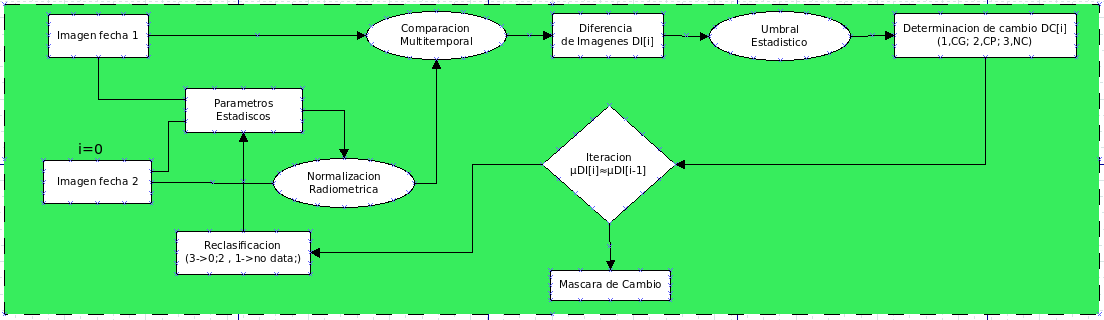
\includegraphics[width=0.8\linewidth, height=0.5\textheight]{imagenes/iteracion}
\caption{Diagrama de iteraci\'on}
\label{fig:iteracion}
\end{figure}


\end{frame}


%------------------------------------------------
\begin{frame}
	\frametitle{Metodolog\'ia - Post-Proceso}
	\textbf{C\'alculo de Carbono}\\~\\	
	En base al mapa global de carbono correspondiente a Saatchi y a nuestro c\'alculo de NDVI de la misma fecha, se realizo un muestro observando una correlaci\'on. De esta forma es posible hallar una funci\'on lineal que convierta el NDVI a carbono.
	
\end{frame}

%------------------------------------------------
\begin{frame}
	\frametitle{Metodolog\'ia - Post-Proceso}
	\textbf{Muestreo con 240 puntos aleatorios del a\~{n}o 2001}\\~\\	
	\begin{figure}
		\centering
		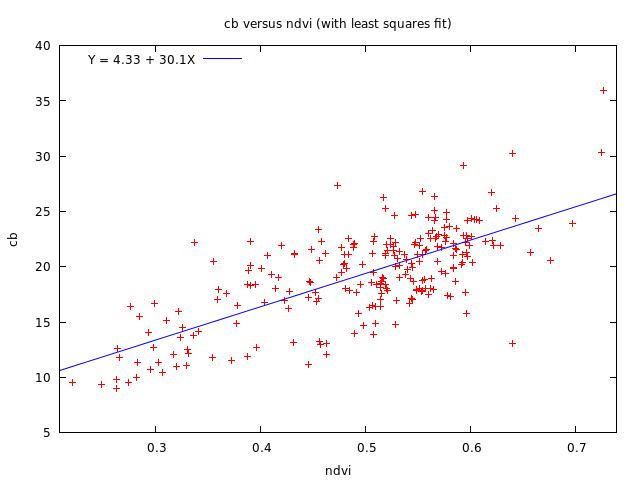
\includegraphics[width=0.7\linewidth, height=0.6\textheight]{imagenes/ndviCarb}
		\caption{Regresi\'on Lineal con r2= 0.509125 (moderado)}
		\label{fig:ndviCarb}
	\end{figure}
	
	
\end{frame}




%------------------------------------------------

%------------------------------------------------
\begin{frame}
	\frametitle{Pruebas experimentales}
	\textbf{Evaluaci\'on de los resultados y control de calidad}\\~\\	
Se realizaron el calculo del porcentaje de precisi\'on global y el coeficiente Kappa.
	
\end{frame}

%------------------------------------------------
\begin{frame}
	\frametitle{Metodolog\'ia - Post-Proceso}

% Please add the following required packages to your document preamble:
% If you use beamer only pass "xcolor=table" option, i.e. \documentclass[xcolor=table]{beamer}
\begin{table}[]
	\centering
	\begin{tabular}{|c|l|l|l|l|}
		\hline
		\rowcolor[HTML]{FFFFC7} 
		\multicolumn{1}{|l|}{\cellcolor[HTML]{FFFFC7}Coeficiente de tolerancia} & Zona   & GA        & Coef. Kappa & Puntos  \\ \hline
		& Urbana & 84.177819 & 0.474973    & 2835532 \\ \cline{2-5} 
		& Rural  & 93.874461 & 0.659546    & 3190560 \\ \cline{2-5} 
		\multirow{-3}{*}{N=1}                                                   & Humeda & 90.603407 & 0.299295    & 1865591 \\ \hline
		& Urbana & 83.47319  & 0.314602    & 2835532 \\ \cline{2-5} 
		& Rural  & 94.921675 & 0.673034    & 3190560 \\ \cline{2-5} 
		\multirow{-3}{*}{N=1.5}                                                 & Humeda & 95.278279 & 0.42258     & 1865591 \\ \hline
		& Urbana & 81.630537 & 0.093501    & 2835532 \\ \cline{2-5} 
		& Rural  & 94.334537 & 0.571205    & 3190560 \\ \cline{2-5} 
		\multirow{-3}{*}{N=2}                                                   & Humeda & 96.68802  & 0.425243    & 1865591 \\ \hline
	\end{tabular}
	\caption{Resultados de validaci\'on}
	\label{my-label}
\end{table}
	
\end{frame}


\begin{frame}
\Huge{\centerline{Gracias}}
\end{frame}

%----------------------------------------------------------------------------------------

\end{document} 